\begin{abstract}
Whether a language model solves grade school arithmetic by reasoning or by reproducing
training data is normally unanswerable, because the pretraining corpora of the models being
measured are closed. Instella publishes its complete mixture, and its stage two synthetic
component derives from the GSM8K training split rather than the test split, so exposure
becomes a measured property fixed by exact thirteen gram containment instead of an estimated
one. Against the full released pool of 1{,}367{,}882 rows no GSM8K test item reaches
containment 0.50 and the maximum observed is 0.487, establishing that benchmark performance
on that split is not recovered text. A premise deletion probe over 3179 variants across 1779
parent problems then asks what the model does when a problem no longer determines an answer.
Under the standard answer forcing prompt it emits a confident number on 92.5 percent of
provably underdetermined items. Under a prompt differing only in naming abstention as an
option it declines on 53.8 percent of them while declining on 1.1 percent of the untouched
answerable parents, a discrimination of $+52.63$ points on $[+50.77, +54.57]$ that grows
monotonically across the training pipeline from $+1.84$ at stage one through $+10.10$ and
$+38.08$ to instruct, with wrong refusals never exceeding 3.5 percent at any stage.
Discrimination is graded by reasoning depth: abstention on underdetermined problems falls
$5.22$ points per additional calculator step while the answerable control stays flat at
$-0.11$, a difference of $-5.11$ on $[-6.36, -3.82]$, and the decay steepens as the
checkpoint improves. Controlled injection at a fixed 8{,}388{,}608 token budget separates
what heavy exposure returns from what it does not: at sixty four repetitions, verbatim
reproduction of injected documents reaches 0.946 and the memorised calculation chain returns
at $+5.44$ points on $[+1.46, +9.38]$, while the final answer does not, at $+1.52$ on
$[-2.12, +5.20]$. The answer result replicates on OLMo-2-1B, Qwen2.5-1.5B and Qwen2.5-3B
across fifteen dose points, including a model driven to verbatim 1.000. Competent procedure
execution and verification of premise sufficiency are therefore separable capabilities, the
second emerging later in training and decaying with the depth of the chain being tracked.
\end{abstract}

\section{Introduction}

A model that answers grade school arithmetic correctly may be reasoning about the premises it
is given or reproducing text it has seen. Distinguishing the two normally requires knowing
what the model read, and the corpora of the models under test are closed, so the question is
usually approached through proxies such as perplexity signatures or benchmark rewriting.
Instella~\citep{instella2025} removes the obstacle. Its complete pretraining mixture is
released, and the stage two synthetic component is generated from the GSM8K training
split~\citep{cobbe2021gsm8k} rather than the test split, so exposure is measurable per item.

That measurement comes first because everything after it depends on the answer. Against the
full released pool of 1{,}367{,}882 rows, no GSM8K test item reaches thirteen gram
containment 0.50, and the highest value observed anywhere is 0.487. Performance on the test
split is therefore not recovered text, and the split can be used as an exposure contrast
rather than merely a difficulty contrast.

With that established, the question becomes what the reasoning consists of. A premise
deletion probe removes exactly one premise that the reference solution consumes, leaving a
problem whose stated answer is no longer derivable. Two things can then be measured on the
same items: whether the model notices, and whether exposure to the original changes what it
produces.

Both answers are informative and they point in different directions. The model does detect
insufficiency, the ability strengthens through every stage of training, and it decays
predictably as the reasoning chain lengthens. Heavy exposure returns the memorised
calculation chain but not the final answer, a dissociation that holds under a controlled
intervention and replicates across three further model families.

\section{Setup}

\paragraph{Exposure.} Containment is the fraction of an item's thirteen grams appearing in a
single corpus document, taking the maximum over documents. The subset consumed during stage
two, \texttt{train\_119K}, holds 119{,}014 rows; the full released pool holds 1{,}367{,}882.
Measured on identical items through one extraction path, 9.65 percent of GSM8K train parents
reach containment 0.999 or above against the consumed subset and 18.52 percent against the
pool, so the pool overstates exposure and the consumed subset is the correct reference.

\paragraph{The probe.} Each item removes one premise the reference solution consumes,
verified by requiring the annotated calculator chain to depend on it. The result is 3179
variants over 1779 parent problems, split 1591 train and 1588 test. Every item is
underdetermined by construction, so declining is the correct response and any specific number
is wrong.

\paragraph{Checkpoints.} Four public Instella checkpoints span the pipeline: stage one, which
precedes the synthetic corpus, stage two, supervised fine tuning and instruct. Decoding is
greedy and held fixed; base checkpoints are prompted with four exemplars and no chat
template, since a base model loops without them.

\paragraph{Inference.} Intervals are cluster bootstraps over parent problems with 4000 draws
at seed 6198, because several variants can descend from one problem and resampling rows
would understate the interval.

\section{Verification of premise sufficiency}

\subsection{The capability exists and is not prompt compliance}

Under the answer forcing prompt used for benchmark scoring, the model emits a number on 92.5
percent of items that provably do not determine one. Changing only one thing, naming
\texttt{\#\#\#\# unanswerable} as an available response, raises abstention on those items to
53.8 percent at the instruct checkpoint.

That rate alone is ambiguous, because every probe item is underdetermined and a model
offered an escape hatch may simply take it. The control resolves it. Running the identical
prompt and decoding over the untouched parent problems, which are answerable and where
declining is an error, gives an abstention rate of 1.1 percent. The difference,
$+52.63$ points on $[+50.77, +54.57]$, is the quantity of interest: abstention tracks whether
the problem can actually be answered.

\begin{table}[t]
\centering
\caption{Abstention with its control, under a prompt that names abstention as an option.
Pruned items are underdetermined so declining is correct; parent problems are answerable so
declining is an error. Cluster bootstrap over parent problems, 4000 draws, seed 6198.}
\label{tab:abstain}
\small
\begin{tabular}{lcccc}
\toprule
Checkpoint & Declines, underdetermined & Declines, answerable & Discrimination & 95\% CI \\
\midrule
Stage 1     & 0.043 & 0.025 & $+1.84$  & $[+0.97, +2.70]$ \\
Instella 3B & 0.110 & 0.008 & $+10.10$ & $[+8.94, +11.30]$ \\
SFT         & 0.416 & 0.035 & $+38.08$ & $[+36.06, +40.02]$ \\
Instruct    & 0.538 & 0.011 & $\mathbf{+52.63}$ & $[+50.77, +54.57]$ \\
\bottomrule
\end{tabular}
\end{table}

Table~\ref{tab:abstain} shows the capability developing across the pipeline. Stage one, which
precedes the synthetic corpus entirely, discriminates by less than two points. Each
subsequent stage improves it, and wrong refusals on answerable problems never exceed 3.5
percent, so the gain does not come from a growing willingness to decline.

\subsection{Discrimination decays with reasoning depth}

The capability is not uniform over problems. Figure~\ref{fig:abstain} plots abstention
against the length of the reference solution's calculator chain. On underdetermined problems
at the instruct checkpoint the rate falls from 0.623 at one step to 0.364 at seven, a slope
of $-5.22$ points per step. On the answerable control the slope is $-0.11$ with an interval
containing zero, so the pattern is not a tendency to decline more on short problems. The
difference of slopes is $-5.11$ on $[-6.36, -3.82]$.

\begin{figure}[t]
\centering
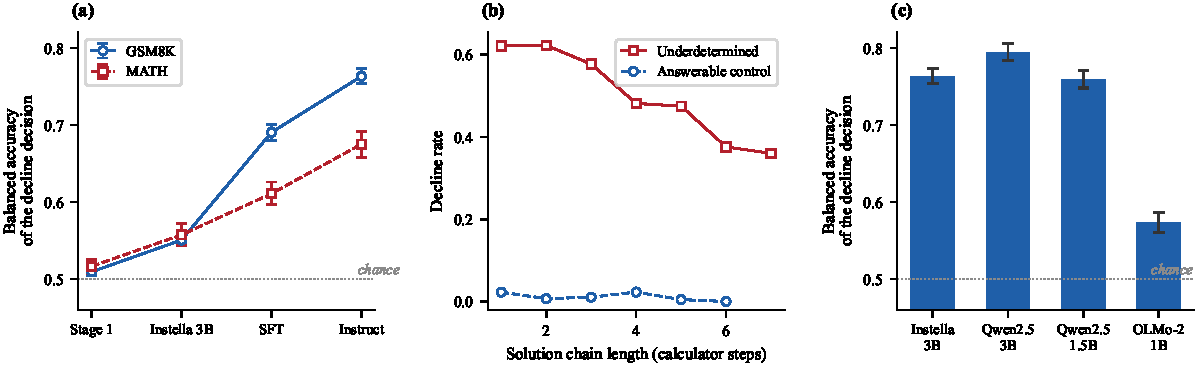
\includegraphics[width=\linewidth]{mathai_fig_abstention.pdf}
\caption{Left: discrimination between underdetermined and answerable problems across the
training pipeline. Right: abstention against solution chain length at the instruct
checkpoint, with the answerable control on the same axes. The control is flat, so the decay
is specific to detecting that premises are missing.}
\label{fig:abstain}
\end{figure}

The decay steepens as the checkpoint improves, running $-2.34$, $-3.64$ and $-5.11$ for
stage two, supervised fine tuning and instruct. Better models detect insufficiency more often
overall and lose that detection faster as the chain they must track grows longer.
Truncation does not explain it: truncation never exceeds 0.7 percent at any chain length and
restricting to terminated generations reproduces the rates exactly.

\section{What exposure returns}

\subsection{Continued pretraining at controlled doses}

Whether exposure supplies the answer is a causal question, and observation cannot settle it,
so selected items were injected by continued pretraining at five doses under a fixed
8{,}388{,}608 token budget, held constant so that a higher dose displaces filler rather than
buying extra compute. Every arm carries positive controls evaluated before and after: loss on
the injected documents must fall, and the model must continue an injected document verbatim.
A flat dose response with failed controls would measure a broken training run rather than an
absence of memorisation.

Injection worked. Verbatim reproduction climbs from 0.133 with no injection to 0.946 at
sixty four repetitions, while held out document loss rises, confirming the mixture taught
those specific documents rather than the task in general.

\subsection{The chain returns, the answer does not}

Against a never injected control at the same dose, reproduction of the memorised calculation
chain reaches $+5.44$ points on $[+1.46, +9.38]$ at sixty four repetitions and rises
monotonically with dose. Reproduction of the final answer reaches $+1.52$ on
$[-2.12, +5.20]$, an interval containing zero. The model reproduces the source text almost
exactly and still does not recover the deleted quantity or the answer it determines.

The answer result is not specific to Instella. Repeating the identical mixture, budget, seed
and probe on OLMo-2-1B, Qwen2.5-1.5B and Qwen2.5-3B gives $+0.28$, $+0.00$ and $+2.28$
points at the top dose, every interval containing zero, across fifteen dose points in total.
Qwen2.5-3B is the sharpest case: driven to verbatim reproduction of 1.000, complete
reproduction of the injected documents, it recovers the deleted answer no more often than a
model that never saw them.

Reproduction of the chain is established on Instella and not yet established elsewhere. The
three replication models give $+2.42$, $+0.32$ and $-0.30$ points, and testing each against
Instella on shared parent problems fails to separate them in two of three cases, so the
comparison is underpowered rather than contradictory. Whether chain reproduction requires
capacity that a one billion parameter model lacks is open.

\section{Discussion}

Two capabilities that a single accuracy number conflates come apart here. Executing a
solution procedure is present early and improves smoothly. Verifying that the premises
support a solution at all appears later, improves sharply through instruction tuning, and
degrades with the depth of the chain being tracked. A model can be competent at the first
while failing the second, and standard benchmark scoring cannot see the difference because
every item it scores is answerable.

The practical consequence is narrow. Benchmarks built entirely from well posed problems
measure procedure execution and are silent about premise verification, yet deployment
routinely presents underspecified problems. Reporting abstention under a prompt that permits
it, against an answerable control, costs one extra evaluation pass and makes the second
capability visible.

\paragraph{Limitations.} One benchmark domain and one problem generator. Detection is
measured through an explicit abstention option, so a model that recognises insufficiency but
lacks the vocabulary to say so is scored as failing. Chain length correlates with problem
difficulty, and the answerable control rules out a general length effect but not every
difficulty confound. Chain reproduction under injection is established on one model, and the
replication is underpowered for it. Attribution to specific training documents is not
established anywhere.

\paragraph{Conclusion.} Measured against exposure fixed by containment rather than
estimated, Instella's grade school arithmetic performance is not recovered text: no test item
approaches containment against the corpus, and heavy controlled injection returns the
memorised calculation chain without returning the answer. What the probe reveals instead is a
separable capability. The model detects that a problem no longer determines an answer, does
so increasingly well across training, and loses that detection as the reasoning chain
lengthens.
